\documentclass{article}
\usepackage{amsmath}
\usepackage{amsthm}
\usepackage{amssymb}
\usepackage[a4paper, left=1.5cm, right=1.5cm, top=2.5cm, bottom=2.5cm]{geometry}
\usepackage{tikz}
\usetikzlibrary{tikzmark}

\title{HW1}
\author{Li Haolun\ 2022011545}

\begin{document}
\maketitle
\begin{enumerate}
    \item \leavevmode\vadjust{\vspace{-\baselineskip}}\newline
    \begin{figure}[!h]
        \centering
        \begin{tikzpicture}
            \draw[->] (0,0) -- (2,0) node[right] {$x_1$};
            \draw[->] (0,0) -- (0,2) node[above] {$x_2$};
            \draw[domain=0.5:1.5, samples=100] plot (\x, {-\x+2});
        \end{tikzpicture}
    \end{figure}
    \item \begin{proof}
        Since the goods for 2 curves are the same, the relative price of the goods is the same.\par
        Therefore, the slope of the 2 curves are the same, which means the 2 curves are parallel.
    \end{proof}
    \item 
    \begin{equation}
        \begin{aligned}
            U
            &=3(x_1^2+2x_1x_2+x_2^2)+10 \\
            &=3(x_1+x_2)^2+10 \\
            \Rightarrow\sqrt{\frac{U-10}{3}}
            &=x_1+x_2
        \end{aligned} \nonumber
    \end{equation}
    \begin{figure}[!h]
        \centering
        \begin{tikzpicture}
            \draw[->] (0,0) -- (2,0) node[right] {$x_1$};
            \draw[->] (0,0) -- (0,2) node[above] {$x_2$};
            \draw[domain=0.5:1.5, samples=100] plot (\x, {-\x+2});
        \end{tikzpicture}
    \end{figure}\par
    It is the preference of substitutes.
    \item \begin{enumerate}
        \item[(1)] \begin{proof}
            For perfect substitutes, a consumer is willing to substitute one good for the other at a constant rate.\par
            So, 
            \begin{equation}
                \begin{aligned}
                    \frac{\partial x_2}{\partial x_1}
                    &=\frac{\partial U}{\partial x_1}/\frac{\partial U}{\partial x_2} \\
                    &=\frac{\frac{1}{\rho}(\alpha_1x_1^{\rho}+\alpha_2x_2^{\rho})^{\frac{1}{\rho}-1}\alpha_1\rho x_1^{\rho-1}}{\frac{1}{\rho}(\alpha_1x_1^{\rho}+\alpha_2x_2^{\rho})^{\frac{1}{\rho}-1}\alpha_2\rho x_2^{\rho-1}} \\
                    &=\frac{\alpha_1}{\alpha_2}(\frac{x_1}{x_2})^{\rho-1} \\
                    &=\text{constant rate}
                \end{aligned} \nonumber
            \end{equation}
        \end{proof}
        It's clear that $\frac{\alpha_1}{\alpha_2}(\frac{x_1}{x_2})^{\rho-1}$ is constant if and only if $\rho=1$.
        \item[(2)] \begin{proof}
            For perfect complements, a consumer always consumes commodities 1 and 2 in fixed proportion.\par
            So, 
            \begin{equation}
                \begin{aligned}
                    \frac{\partial x_2}{\partial x_1}
                    &=\frac{\partial U}{\partial x_1}/\frac{\partial U}{\partial x_2} \\
                    &=\frac{\alpha_1}{\alpha_2}(\frac{x_1}{x_2})^{\rho-1} \\
                    &=0\text{ or }\infty
                \end{aligned} \nonumber
            \end{equation}
        \end{proof}
        It's clear that $\frac{\alpha_1}{\alpha_2}(\frac{x_1}{x_2})^{\rho-1}=0\text{ or }\infty$ if and only if $\rho=-\infty$.
        \item[(3)] For Cobb-Douglas,
        \begin{equation}
            \begin{aligned}
                \frac{\partial x_2}{\partial x_1}
                &=\frac{\partial U}{\partial x_1}/\frac{\partial U}{\partial x_2} \\
                &=\frac{\alpha_1}{\alpha_2}(\frac{x_1}{x_2})^{\rho-1} \\
                &\propto\frac{x_2}{x_1}
            \end{aligned} \nonumber
        \end{equation}
        So, $\rho=0$.
    \end{enumerate}
    \item \begin{enumerate}
        \item[(1)] \leavevmode\vadjust{\vspace{-\baselineskip}}\newline
        \begin{figure}[!h]
            \centering
            \begin{tikzpicture}
                \draw[->] (0,0) -- (2,0) node[right] {$x$};
                \draw[->] (0,0) -- (0,2) node[above] {$y$};
                \draw[domain=0.2:2/3, samples=100] plot (\x, {-2*\x+2});
                \draw[domain=2/3:1.8, samples=100] plot (\x, {-0.5*\x+1});
            \end{tikzpicture}
        \end{figure}
        \item[(2)] \leavevmode\vadjust{\vspace{-\baselineskip}}\newline
        \begin{figure}[!h]
            \centering
            \begin{tikzpicture}
                \draw[->] (0,0) -- (2,0) node[right] {$x$};
                \draw[->] (0,0) -- (0,2) node[above] {$y$};
                \draw[domain=0.2:1, samples=100] plot (\x, {-\x+2});
                \draw[domain=1:1.8, samples=100] plot (\x, {1});
            \end{tikzpicture}
        \end{figure}
        \item[(3)] \leavevmode\vadjust{\vspace{-\baselineskip}}\newline
        \begin{figure}[!h]
            \centering
            \begin{tikzpicture}
                \draw[->] (0,0) -- (2,0) node[right] {$x$};
                \draw[->] (0,0) -- (0,2) node[above] {$y$};
                \draw[domain=0.2:1/3, samples=100] plot (\x, {-4*\x+2});
                \draw[domain=1/3:2/3, samples=100] plot (\x, {-\x+1});
                \draw[domain=2/3:1.8, samples=100] plot (\x, {-0.25*\x+0.5});
            \end{tikzpicture}
        \end{figure}
    \end{enumerate}
    \item 
    \begin{equation}
        \begin{aligned}
            25x+15y&=C \\
            U&=\min(x,y^2) \\
            \Rightarrow U&=\min(\frac{C-15y}{25},y^2) \\
        \end{aligned} \nonumber
    \end{equation}
    So, when $y=7$, we have
    \begin{equation}
        \frac{C-15y}{25}=y^2 \nonumber
    \end{equation}
    \begin{equation}
        \Rightarrow C=1330 \nonumber
    \end{equation}
    \item 
    \begin{equation}
        \begin{aligned}
            U&=x_1+\sqrt{x_2+x_3} \\
            x_1&+2x_2+3x_3=100 \\
            \Rightarrow U&=100-2x_2-3x_3+\sqrt{x_2+x_3} \\
        \end{aligned} \nonumber
    \end{equation}
    For $x_2,x_3>0$:
    \begin{equation}
        \begin{aligned}
            \frac{\partial U}{\partial x_2}
            &=\frac{1}{2\sqrt{x_2+x_3}}-2 \\
            &=0 \\
            \Rightarrow x_2&=\frac{1}{16}-x_3
        \end{aligned} \nonumber
    \end{equation}
    \begin{equation}
        \begin{aligned}
            \frac{\partial U}{\partial x_3}
            &=\frac{1}{2\sqrt{x_2+x_3}}-3 \\
            &=0 \\
            \Rightarrow x_3&=\frac{1}{36}-x_2
        \end{aligned} \nonumber
    \end{equation}
    There's no solution for $x_2,x_3>0$.\par
    Then consider $x_2=0$:
    \begin{equation}
        \begin{aligned}
            U&=100-3x_3+\sqrt{x_3} \\
            \frac{\partial U}{\partial x_3}
            &=\frac{1}{2\sqrt{x_3}}-3 \\
            &=0 \\
            \Rightarrow x_3&=\frac{1}{36} \\
            x_1&=\frac{1199}{12} \\
            U&=100\frac{1}{12}
        \end{aligned} \nonumber
    \end{equation}
    $x_3=0$:
    \begin{equation}
        \begin{aligned}
            \Rightarrow x_2&=\frac{1}{16} \\
            x_1&=\frac{799}{8} \\
            U&=100\frac{1}{8}
        \end{aligned} \nonumber
    \end{equation}
    So, the optimal choice should be $x_1=\frac{799}{8},x_2=\frac{1}{16},x_3=0$.\par
    But $x_i$ are integer, so the optimal choice is $x_1=100,x_2=0,x_3=0$. And $U=100$.
    \item 
    \leavevmode\vadjust{\vspace{-\baselineskip}}
    \begin{figure}[!h]
        \centering
        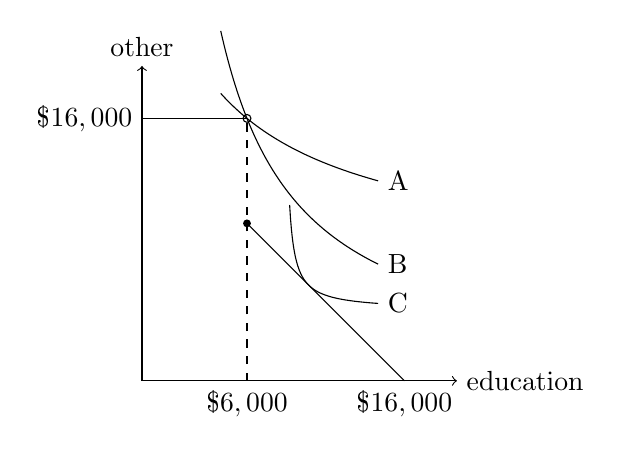
\begin{tikzpicture}
            \draw[->] (0,0) -- (4,0) node[right] {education};
            \draw[->] (0,0) -- (0,4) node[above] {other};
            \draw[dashed] (4/3,0) node[below]{\$$6,000$} -- (4/3,10/3);
            \draw (4/3, 10/3) -- (0, 10/3) node[anchor=east] {\$$16,000$};
            \draw (4/3, 2) -- (10/3, 0) node[anchor=north] {\$$16,000$};
            \draw (4/3, 10/3) circle (0.05);
            \fill (4/3, 2) circle (0.05);
            \draw[domain=1:3, samples=100] plot (\x, {(40/9)/(\x+1)+(10/7)}) node[anchor=west] {A};
            \draw[domain=1:3, samples=100] plot (\x, {(40/9)/\x}) node[anchor=west] {B};
            \draw[domain=1.875:3, samples=100] plot (\x, {0.1/(\x-1.8)+0.9}) node[anchor=west] {C};
        \end{tikzpicture}
    \end{figure}
    \item 
    \begin{enumerate}
        \item[(1)] \begin{equation}
            \begin{aligned}
                x+y&=600 \\
                U
                &=x^{0.1}y^{0.9}\\
                -\frac{\partial y}{\partial x}
                &=-\frac{\partial U}{\partial x}/\frac{\partial U}{\partial y} \\
                &=-\frac{0.1x^{-0.9}y^{0.9}}{0.9x^{0.1}y^{-0.1}} \\
                &=-\frac{y}{9x} \\
                &=-1 \\
                \Rightarrow y&=9x \\
                \Rightarrow x&=60 \\
                y&=540 \\
            \end{aligned} \nonumber
        \end{equation}
        \item[(2)] \begin{equation}
            \begin{aligned}
                x+y&=600+100=700 \\
                y&=9x \\
                \Rightarrow x&=70 \\
                y&=630 \\
            \end{aligned} \nonumber
        \end{equation}
        \item[(3)] \begin{equation}
            \begin{aligned}
                \frac{1}{2}x+y&=600 \\
                \frac{\partial y}{\partial x}
                &=-\frac{y}{9x} \\
                &=-\frac{1}{2} \\
                \Rightarrow 2y&=9x \\
                \Rightarrow x&=120 \\
                y&=540 \\
            \end{aligned} \nonumber
        \end{equation}
        \item[(4)] \begin{equation}
            \begin{cases}
                y=600 &(0\leq x<100) \\
                (x-100)+y=600 &(x\geq100) \\
            \end{cases} \nonumber
        \end{equation}
        \begin{equation}
            \begin{aligned}
                \frac{\partial y}{\partial x}
                &=-\frac{y}{9x} \\
                &=-1 (x\leq100) \\
                \Rightarrow y&=9x(x\geq100) \\
                \Rightarrow x&=100 \\
                y&=600 \\
            \end{aligned} \nonumber
        \end{equation}
        If there's a black market,
        \begin{equation}
            \begin{cases}
                0.8x+y=680 &(0\geq x<100) \\
                (x-100)+y=600 &(x\geq100) \\
            \end{cases} \nonumber
        \end{equation}
        \begin{equation}
            \begin{cases}
                y=7.2x &(0\geq x<100) \\
                y=9x &(x\geq100) \\
            \end{cases} \nonumber
        \end{equation}
        \begin{equation}
            \begin{aligned}
                \Rightarrow x&=85 \\
                y&=612 \\
            \end{aligned} \nonumber
        \end{equation}
    \end{enumerate}
    \item 
    \begin{enumerate}
        \item[(1)] 
            \begin{equation}
                C+8R=160 \nonumber
            \end{equation}
        \item[(2)] 
        \begin{equation}
            \begin{aligned}
                -\frac{\partial C}{\partial R}
                &=-\frac{\partial U}{\partial R}/\frac{\partial U}{\partial C} \\
                &=-\frac{C}{R} \\
                &=-8 \\
                \Rightarrow C&=8R \\
                \Rightarrow R&=10 \\
                C&=80 \\
            \end{aligned} \nonumber
        \end{equation}
        \item[(3)] 
        \begin{equation}
            C+12R=232 \nonumber
        \end{equation}
        \begin{equation}
            \begin{aligned}
                C&=12R \\
                \Rightarrow R&=\frac{29}{3} \\
                C&=116 \\
            \end{aligned} \nonumber
        \end{equation}
        \item[(4)] 
        \begin{equation}
            \begin{cases}
                C+4R=112 &(R<12) \\
                C+8R=160 &(R\geq12) \\
            \end{cases} \nonumber
        \end{equation}
        \begin{equation}
            \begin{aligned}
                C&=8R \\
                \Rightarrow R&=12 \\
                C&=96 \\
            \end{aligned} \nonumber
        \end{equation}
    \end{enumerate}
\end{enumerate}
\end{document}